
%%% BEGIN APPENDIX %%%
%% move this to input after done editing
%% Appendix chapter %%

\begin{subappendices}

\section{Continuous representation of single-cell expression profiles through dimensionality reduction}

Following our hierarchical clustering analysis of single ILC precursor expression profiles, we aimed to develop a more precise characterization of the developmental relationships between individual expression profiles. Initially, we focused on improving our treatment of filtering and normalization routines for single-cell multiplex qPCR data to achieve more accurate expression comparisons. Next, applied a non-linear dimensionality reduction technique to our revised expression profiles to illustrate the continuous developmental trajectory structure in our data and enhance our interpretation of ILC differentiation.

\subsection{Revisited filtering and normalization for single-cell multiplex qPCR}

Standard methods for interpreting expression measurements from quantitative real-time PCR (qPCR) data rely on comparison to a set of common housekeeping gene standards. qPCR measurements report the number of PCR amplification cycles required for a transcript to reach a pre-specified threshold level. The cycle number for a given transcript is then compared to the cycle number associated with a housekeeping gene to report a relative measure of gene expression. Specifically, these cycle number thresholds are typically subtracted to produce a logarithmic scale expression measure called $\Delta$Ct, or the change in cycle thresholds. Single-cell multiplex qPCR perform tens of qPCR measurements in parallel from transcript material portioned from single cells.

Due to the small amount of starting material used in single-cell multiplex qPCR experiments, it is not surprising that measurement preparation could fail entirely for individual cells. In these experiments, typically a few housekeeping genes are measured and cells are filtered if they contain a failed measurement for any housekeeping gene. In our experiment, we measured three housekeeping genes, \textit{Actb}, \textit{Gapdh}, and \textit{Hprt}, and found that this filtering metric is not always the most representative of outlier expression profiles. For some cells, expression measurements appear to be within normal ranges but a single housekeeping gene happens to be missing. Instead of relying on accurate measurement of only three housekeeping genes, we instead filter outlier cells based on extreme shifts in expression and low gene coverage. Specifically, when we plot the proportion of total genes expressed by the median z-scaled deviation in expression for measured genes for each cell, we clearly find outliers with low gene coverage and large shifts in measured expression that correspond to failed measurement (Figure \ref{fig:app_filtnorm}A). We also observe some cells that have large shifts in measured expression despite having relatively normal gene coverage. We assume these cells were simply measured with reduced efficiency and that normalization procedures can regularize their expression values. We expect this filtering procedure is more robust than using a strict housekeeping gene requirement and retains some cells where a housekeeping gene measurement failed sporadically. 

%% Appendix Figure 1 Filtering and Normalization %%
\begin{figure}[p]
	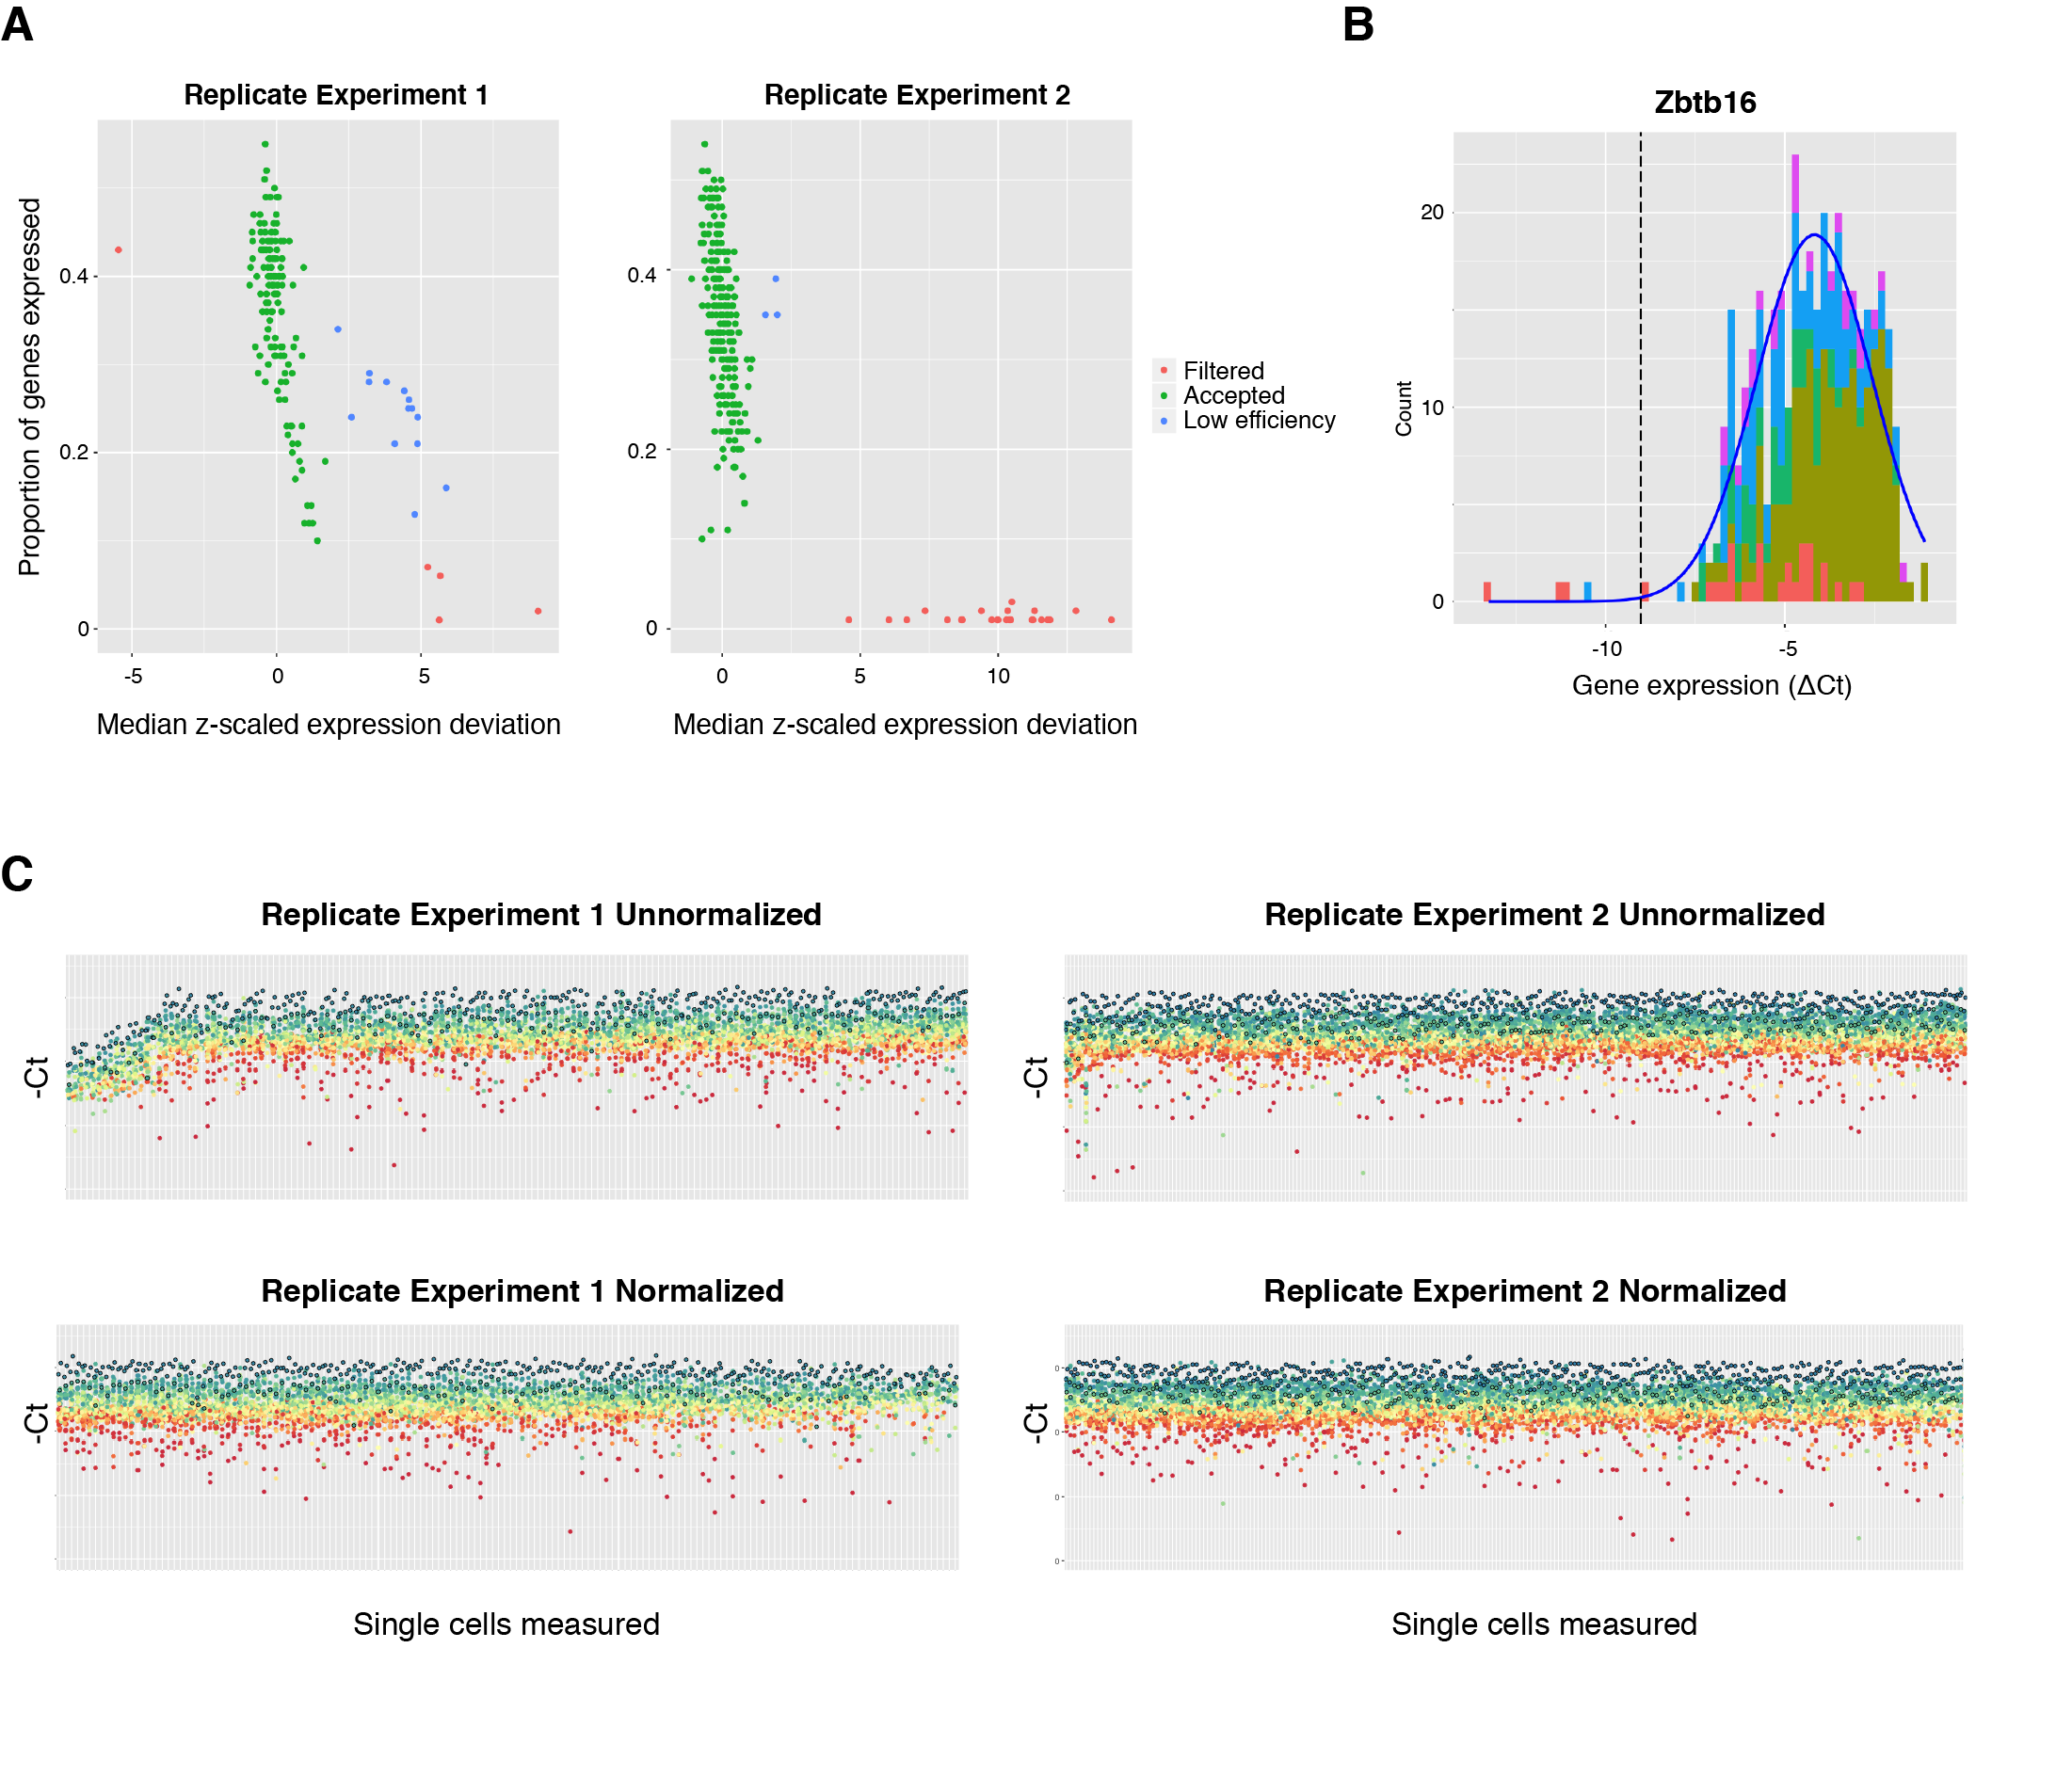
\includegraphics[width=\textwidth]{figures/appendix/Appendix_1_filtering_normalization}
	\caption{Data-driven single-cell multiplex qPCR filtering and normalization.} 
	A) Outlier cells were filtered if they had low gene coverage and large shifts in gene expression measurements. ‘Low efficiency’ cells with normal gene coverage but large shifts in gene expression measurements were retained for further analysis. B) Distribution of measured $\Delta$Ct values for \textit{Zbtb16} with Gaussian fit shown in blue and low expression threshold ($\mu - 3\sigma$) shown by the dotted line. Colors distinguish separate experiments. C) Regression model based normalization corrects for large shifts in gene expression. Scatterplot of measured expression values (--Ct) shown for each cell before and after normalization. Colors correspond to different genes.
	\label{fig:app_filtnorm}
\end{figure}

The most basic normalization strategy drawn from low throughput qPCR measurements is to report expression levels relative to housekeeping gene expression level. This strategy relies on accurate measurement of relatively few housekeeping genes as well as the assumption of their stable expression and fails to incorporate additional expression information from the large number of other genes measured. For high-throughput multiplex qPCR experiments, recent normalization methods have been developed based on those used for analysis of bulk expression profiling experiments \cite{mar2009}. However, these methods, such as quantile normalization, tend to produce expression values that are no longer as interpretable in terms of cycle threshold units and may be sensitive large shifts in gene coverage.

We developed a normalization strategy for single-cell multiplex qPCR based on an explicit regression model that accounts for different measurement efficiencies for each cell. Any scaling of the amount of transcript material capable of being measured results in a constant shift in all cycle threshold values measured for a given cell. For all genes with measured expression values in each cell, we fit the following regression model:

\begin{equation}
	Ct_{ij} = X_i + C_j + \varepsilon_i
\end{equation}

Where $Ct_{ij}$ is the cycle threshold measurement for gene $i$ of cell $j$, $X_i$ is the average cycle threshold value for gene $i$, and $C_j$ is the constant shift in measurement efficiency for cell $j$. To obtain normalized expression values, we simply remove the contributions to expression measurements from the cell-specific and experiment specific constants and provide the remaining residual expression variance per gene. The distributions of measured expression values before and after normalization are illustrated in Figure \ref{fig:app_filtnorm}C. 

This procedure is analogous to standard housekeeping gene normalization, but utilizes the complete set of expression information to account for differing measurement efficiencies per cell. Accordingly, we expect this procedure to be more robust to possible inaccuracies in housekeeping gene measurement. We found that this regression-based method reduced measured gene expression variance for many more genes than achieved through housekeeping gene normalization (data not shown). For consistency with standard single-cell qPCR reporting, we calculate final expression values relative to the collective average housekeeping levels for consistency with typically reported expression measurements. This regression-based procedure could produce bias if there is a dominant and consistent shift in most measured expression values between different cell stages. We do not expect this would be a problem if we have a sufficiently diverse representation of genes with different expression dynamics in our assayed panel. This method could be restricted to only use a gene subset with desired distributional properties for further refinement. 

Across all measured cells, the expression values for most genes are normally distributed in Ct with clear outlier values among low expression range, and can be directly seen in the distribution of \textit{Zbtb16} measured values for example (Figure \ref{fig:app_filtnorm}B). It is apparent these outlier values are unphysical, as they purport thousand fold reduction in expression compared to average gene expression levels. To regularize the expression values we use for downstream analysis, for each gene, we iteratively calculate a robust Gaussian fit to the expression value distribution and remove outlier values beyond three standard deviations. We consider removed outlier expression values as equivalent to non-expressed measurements. In the calculation of distance measures between expression profiles, there is the question of how to treat non-expressed measurements relative to measured expression values. This choice effectively determines how we balance a difference in measured expression values to the cost of entirely turning the expression of a gene on or off. For distance metric calculation, we chose to impose a relatively strong penalty for switching gene expression on or off by placing non-expressed measurements 10 Ct below the 3$\sigma$ low expression threshold defined by our Gaussian distribution fits for each gene. This choice is justified since across our data, we found that most expression variance is due to on-off gene expression, even when calculated with non-expressed genes most conservatively placed right at the low expression thresholds. 

\subsection{Dimensionality reduced representation of ILC precursor expression profiles}

We identified a few salient features of our measured population of single cell precursors through hierarchical clustering. We observed dynamic changes in transcription for many genes across ordered developmental stages. In particular, we found a set of transcription factors that are sequentially induced early in ILC specification, as well as a number of transcription factors with transient expression dynamics. Additionally, we found a substantial portion of ILCP showed signs of early lineage differentiation, indicating that within our data the singular developmental path in early ILC specification is branching in later stages. These characteristic properties of a developing precursor population are indicative that representation of this data by a group of discrete clusters may not be the most appropriate. Although we might expect there to be developmental transitions distinguished by induction or downregulation of transcription factors and cell markers, we would expect these transitions should appear to be continuous with sufficient single-cell sampling. In particular, in studying developmental trajectories we don’t expect cell stages to be distinctly well-separated clusters, which is typically assumed in the design of clustering algorithms. Furthermore, clustering metrics often measure the degree of separation between clusters, which makes evaluation of clustering quality between adjacent stages difficult. For these reasons, other methods for interpretation besides a clustering-based approach could be more appropriate for a continuous developmental process. 

Essentially, we would like to reconstruct cellular trajectories that are representative of the neighbor relationships between single-cell expression profiles. Dimensionality reduction techniques are often used to visualize and identify relationships between subgroups in a collection of high-dimensional data; the most commonly applied technique is principal components analysis. Recently, a number of single-cell analysis methods utilize forms of dimensionality reduction to identify the geometries of developmental trajectories and have been further extended to associate individual expression profiles with developmental pseudotime, quantitative measure of biological progression that effectively order transiting cells by developmental stage \cite{trapnell2015}. For our purposes, we apply a non-linear dimensionality reduction technique, t-distributed stochastic neighbor embedding (t-SNE), to illustrate the interpretive benefits a dimensionality reduction-based strategy has in developmental analysis. The aim of t-SNE is to identify a non-linear mapping of data points in a high-dimensional space to points in a low-dimensional space (2D or 3D) in a way that best preserves high-dimensional neighbor relationships in the low-dimensional representation \cite{maaten2008}. Visualization of single-cell population structure has been successfully performed using a technique based on t-SNE \cite{amir2013}. In our case, we expect preservation of local neighbor relationships in a low-dimensional representation will correspond to adjacent placement of developmentally similar precursor cells, and any preservation of longer-range expression profile similarities should reflect the large-scale geometry of developmental trajectories. The balance between preservation of local and long-range cell relationships is controlled by a parameter called the perplexity in t-SNE, and is essentially the extent of neighbor relationships intended to be satisfied in the mapping. 

We calculated the complete set of Euclidean distances between single-cell expression profiles using the normalized and adjusted qPCR expression values as described above and performed t-SNE projection to two dimensions. We found that a perplexity value of 30 was capable of resolving the lineage differentiation and branching structure discussed below. For clarity, mast cell contaminants discussed in the previous chapter are removed from all dimensionality reduction figures presented in this section. 

\subsubsection{RESULTS}

By coloring cells by their assigned hierarchical clusters defined in the previous chapter, it is clear that this continuous representation recapitulates the same developmental progression we previously inferred (Figure \ref{fig:app_clust}A). Specifically, we see a contiguous developmental trajectory that starts with \aLP cluster cells, then transitions through cluster B cells, and is completed by ILCP cluster cells. This continuous representation emphasizes that these cluster transitions appear quite continuous, a feature that could not be easily determined through clustering. It is also apparent that our previously described developmental stages appear to be necessary transition stages that span the primary developmental path. For example, any minimal trajectory from \aLP to ILCP must transit through cluster B, corroborating our previous interpretation of this intermediate stage. Overall, there are no apparent gaps or large jumps between developmental stages, which would indicate potentially missing transition states. This is somewhat surprising given that we know that EILP precursors were not surveyed in our experiment due to their lack of IL-7r expression and might point to the existence of alternative developmental paths. 

%% Appendix Figure 2 Clustering and timing %%
\begin{figure}[p]
	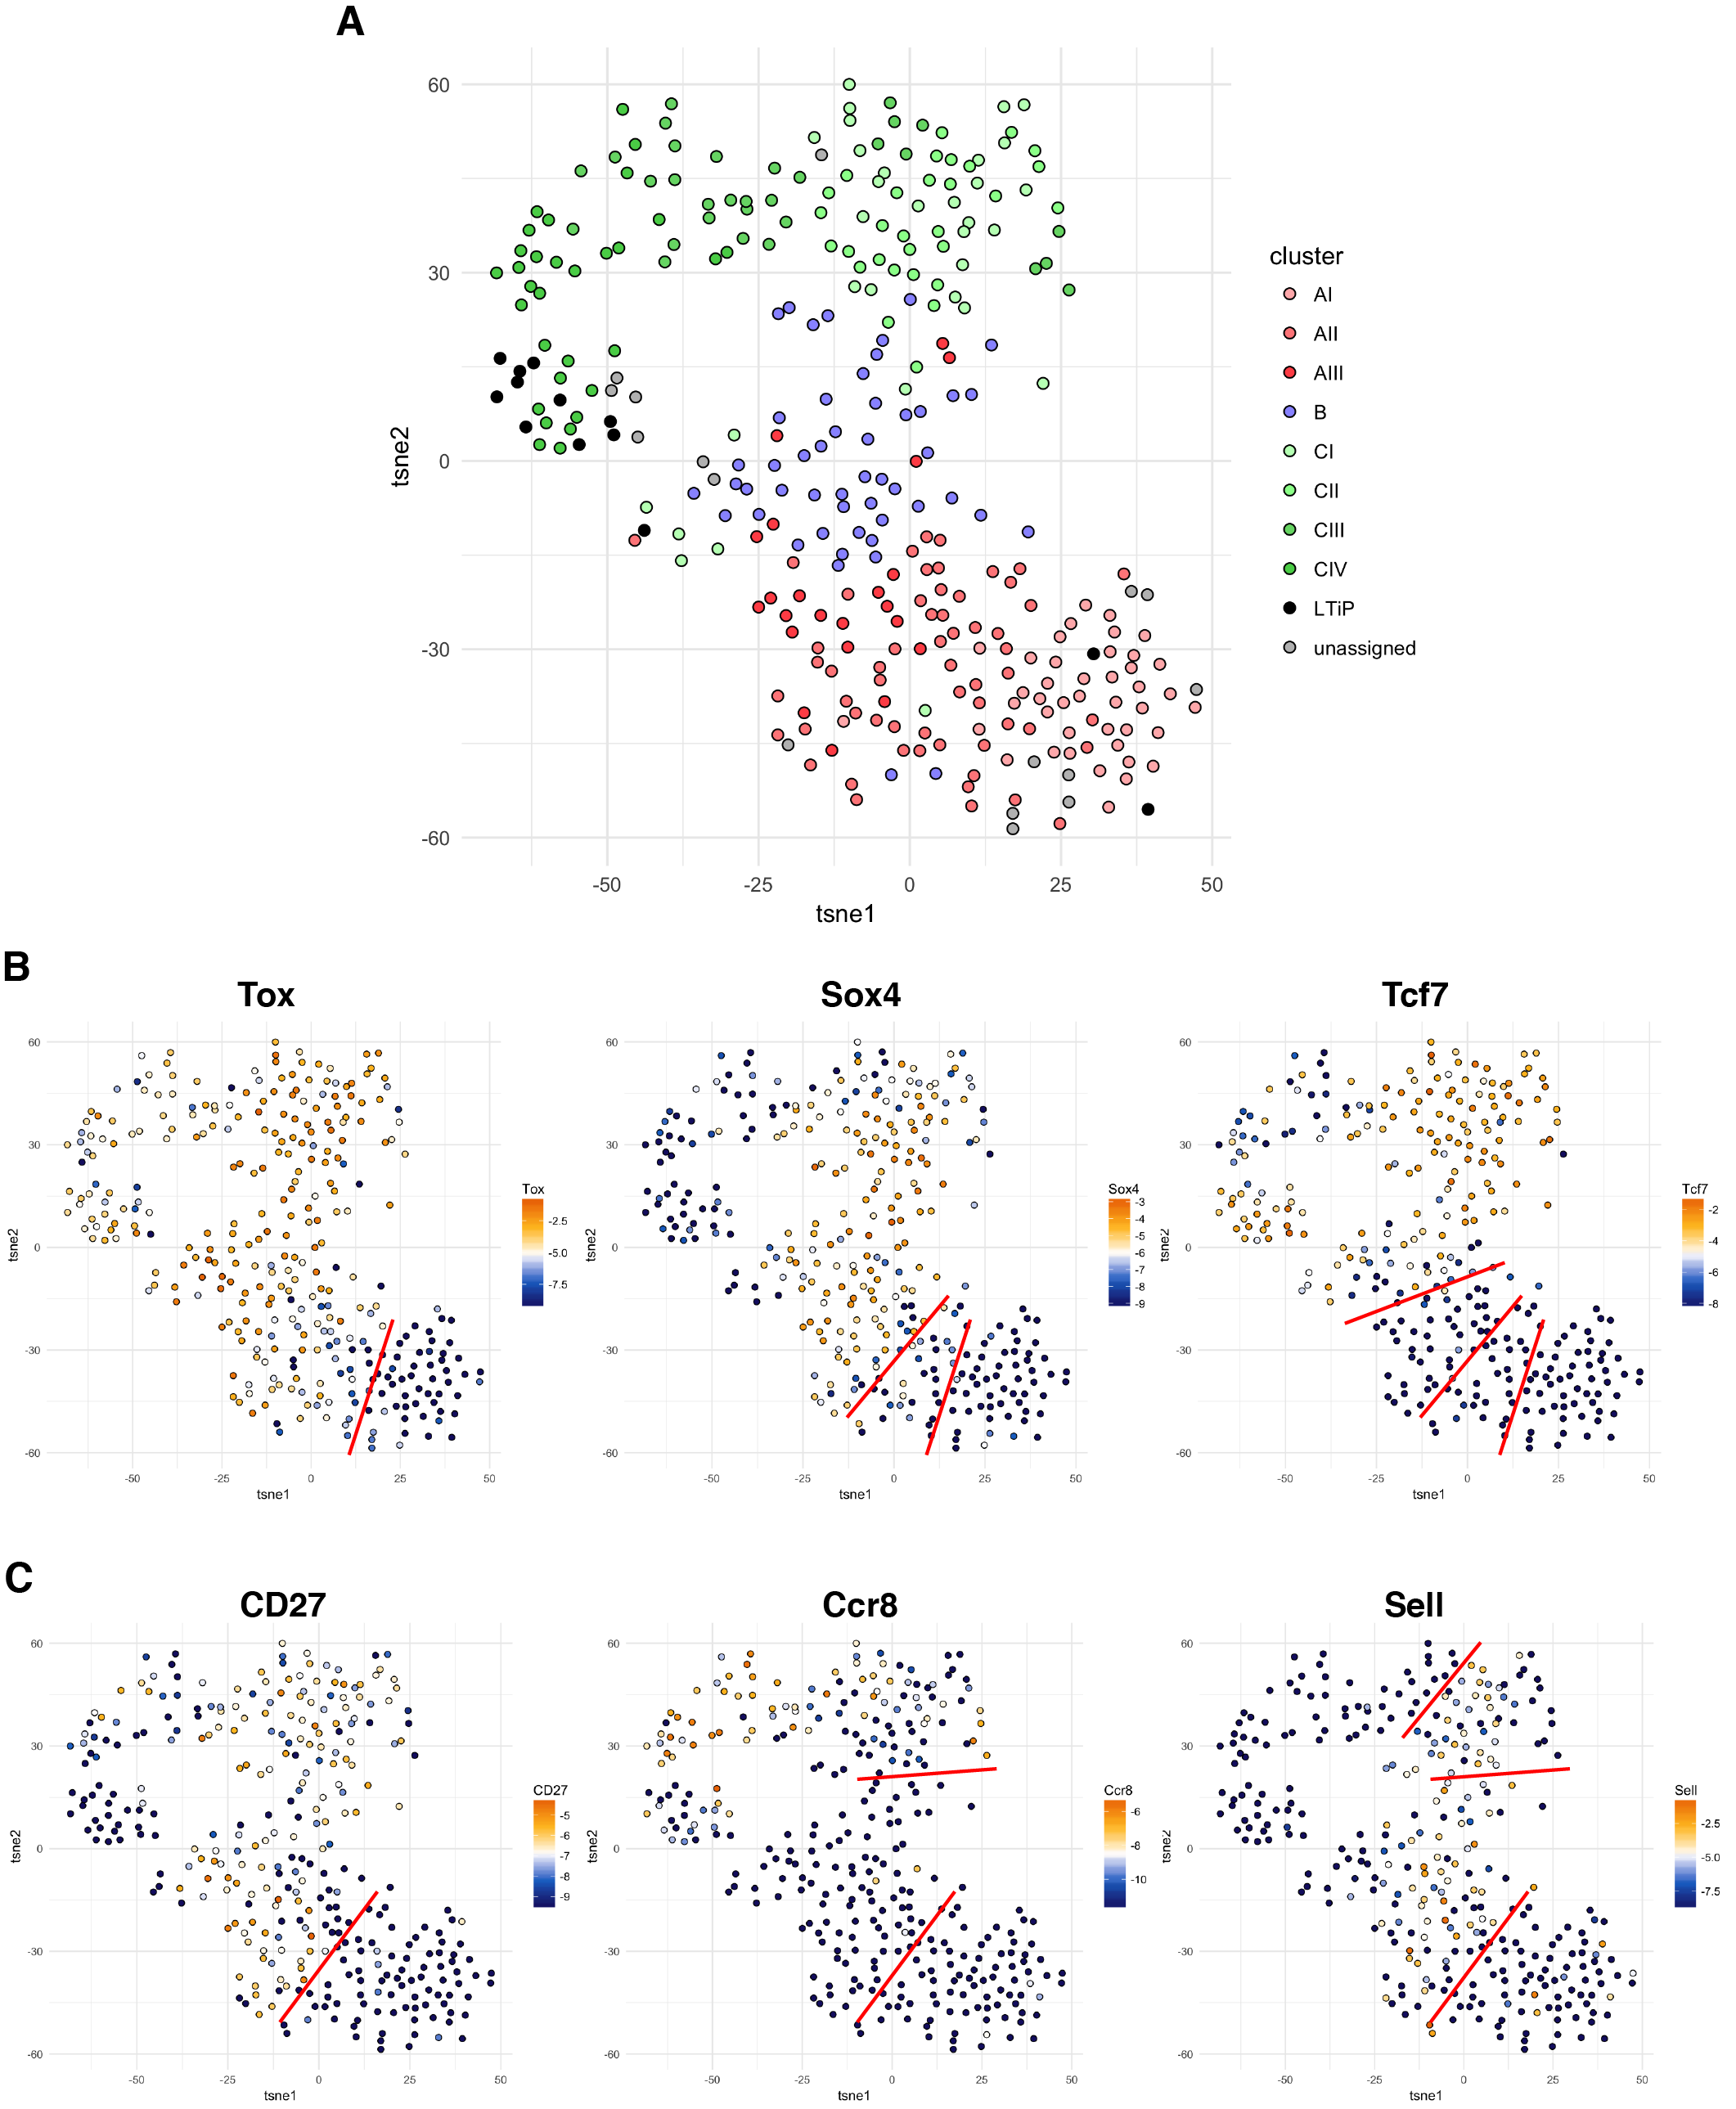
\includegraphics[width=\textwidth]{figures/appendix/Appendix_2_clustering_timing}
	\caption{ILC developmental progression along dimensionality reduced (t-SNE) representation.} 
	A) Continuous developmental representation of ILC precursors with hierarchical clusters colored. B) Sequence of transcription factor induction along primary developmental branch. C) Sequence of surface marker expression along primary developmental branch. Stages of induction highlighted in red. 
	\label{fig:app_clust}
\end{figure}

This continuous developmental representation enables the visualization of gene expression induction without the need to perform precise stage-specific clustering. In a clustering-based approach, improper cluster resolution could be detrimental to the interpretation of developmental progression. If clusters are too large and inclusive, we might average over and effectively miss a transitional stage; on the other hand, if clusters are too small and overfitting, we might erroneously interpret heterogeneity as distinct developmental stages. These concerns are analogous to proper choice of the perplexity parameter in dimensionality reduction by t-SNE, although it is much easier to determine an appropriate range of perplexity values through inspection of the resulting visualizations than it is to determine the most appropriate number of clusters. Accordingly, we expect inference of the relative timing of gene expression induction based on our continuous developmental representation to be less error-prone and more precise. On our continuous representation, by examining the expression \textit{Tcf7}, \textit{Sox4} and \textit{Tox}, we can see the same early sequence of transcription factor induction in \aLP as we had found before but with clear lines of demarcation across the primary developmental branch (Figure \ref{fig:app_clust}B). While the measured cells are destroyed in single-cell expression profiling, these experiments can reveal potential surface markers that delineate developmental stages and are compatible with further experimental manipulation like cell sorting. Among our measured genes, we found that expression of the surface markers \textit{CD27}, \textit{Ccr8}, and \textit{Sell}, tend to have distinct expression patterns along the ILC developmental path (Figure \ref{fig:app_clust}C). The use of these markers could enable better mapping of developmental potential to precursor expression profiles as well as detailed investigation of particular stages in differentiation.

A clearly missing facet in our hierarchical clusters was the resolution of ILC lineage branches. Although we observed early differentiation towards all three types of ILC lineages through direct examination of lineage-defining factors, no hierarchically defined clusters directly corresponded to these distinct lineages. In contrast, these distinct lineage branches are clearly resolved in our continuous developmental representation (Figure \ref{fig:app_branch}A-D). Previously, cells belonging to these differentiating lineages were split between clusters that broadly correspond to earlier and later stages of ILC differentiation after induction of PLZF. Essentially, the gene expression commonalities that correlate with differentiation extent were more dominant in clustering than lineage-specific similarities in gene expression among these cells. Through a two-dimensional continuous representation, we can simultaneously represent developmental progression from earlier to later states of differentiation in concert with divergence between lineage branches. Specifically, we see that expression of \textit{Icos} distinguishes the differentiating ILC2 lineage branch, expression of \textit{Tbx21} distinguishes the differentiating ILC1 lineage branch, and expression of \textit{Rorc} and \textit{Lta} expression distinguishes the differentiating ILC3 branch while simultaneously marking separately sorted LTiP cells. Among differentiating ILCP primed towards the ILC2 lineage, we can observe a variable extent of commitment, where some cells express effector genes such as \textit{Il13} and \textit{Il33r} in addition to \textit{Icos}, \textit{Bcl11b} and \textit{Gata3} (data not shown).

%% Appendix Figure 3 Branching and Multilineage %%
\begin{figure}[p]
	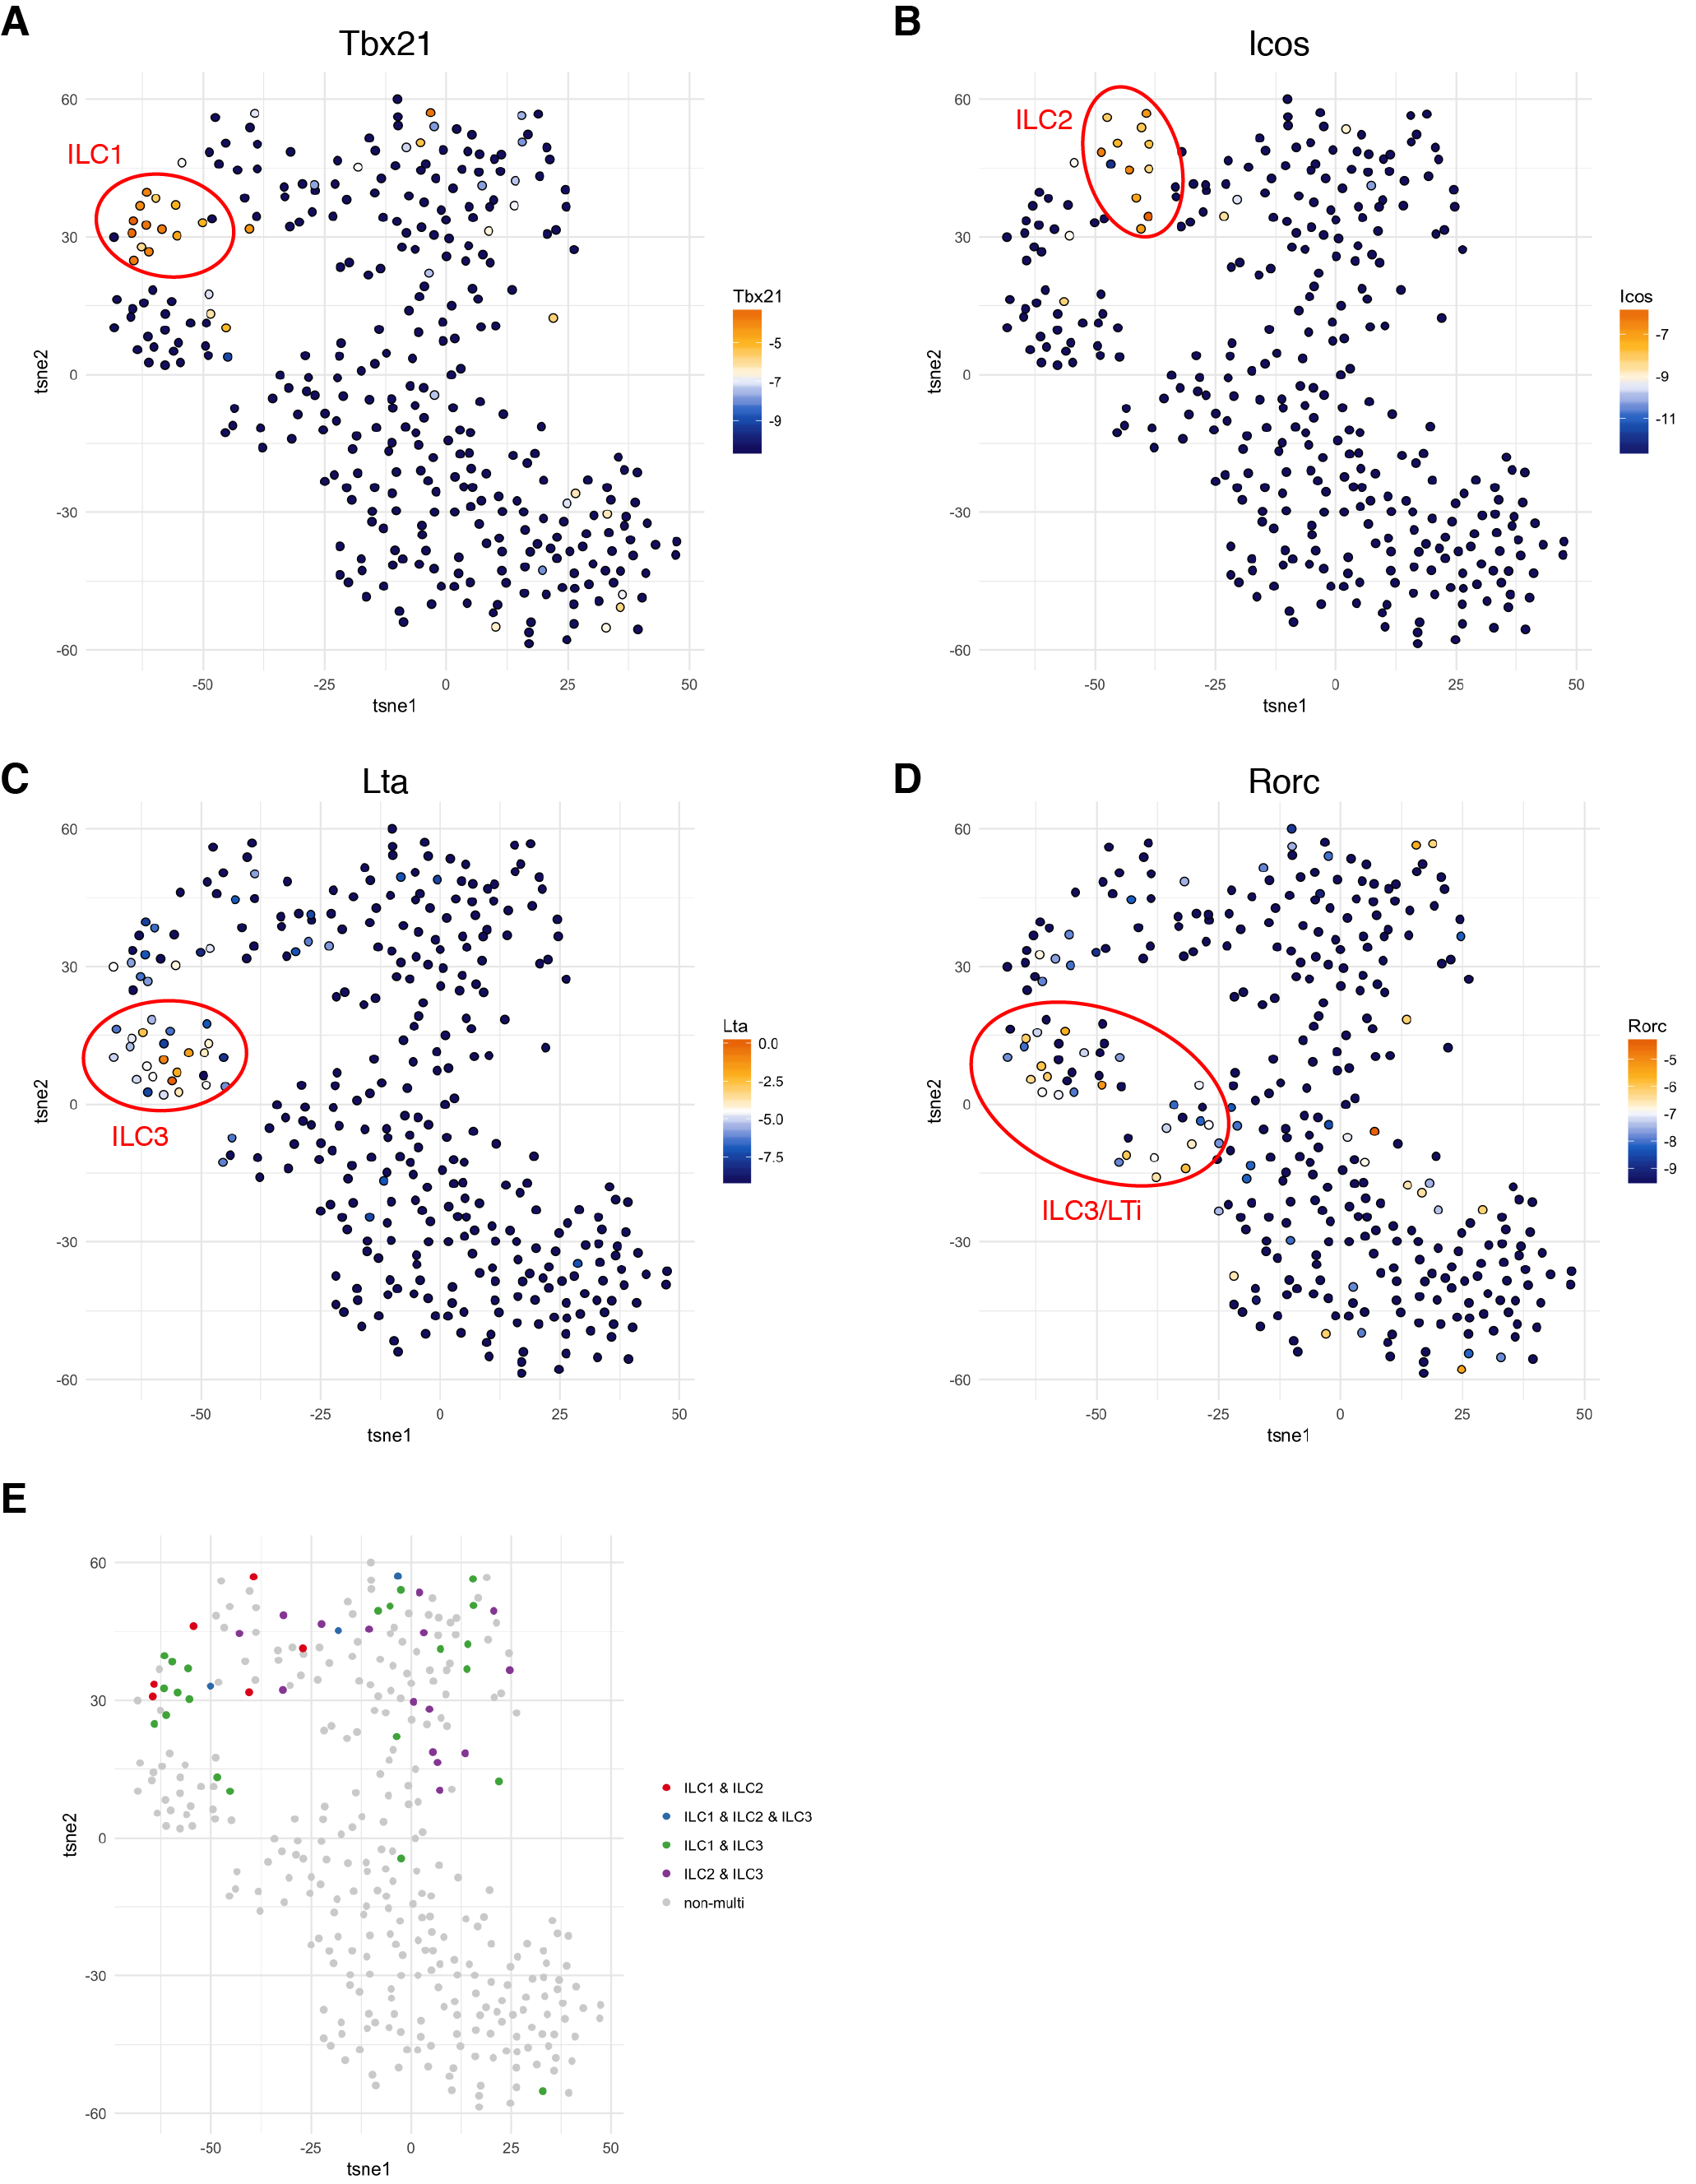
\includegraphics[width=0.9\textwidth]{figures/appendix/Appendix_3_branching_multi}
	\caption{ILC lineage branching on dimensionality reduced (t-SNE) representation.} 
	A-D) Expression of lineage-defining factors identify branching trajectories on continuous developmental representation. Specific lineage branches highlighted in red. E) Multilineage transcriptionally primed ILC precursors are distributed sporadically on ILC developmental path. Colors indicate simulation expression of a specific combination of lineage-defining factors (\textit{Tbx21} for ILC1, \textit{Bcl11b} for ILC2, and \textit{Rorc} for ILC3). 
	\label{fig:app_branch}
\end{figure}


Interestingly, our continuous developmental representation also provides a very direct visualization of branching between the LTi and ILC lineages. In our hierarchical clustering analysis, cells diverging towards the LTi lineage had to be separately extracted from the B cluster population through filtering on a PLZF\UM Tcf7\UP{} signature. In our continuous representation, expression of \textit{Rorc} clearly highlights a protrusion of cells from cluster B diverging from the primary ILC developmental path. Furthermore, this protrusion extends directly towards the differentiated ILC3 and LTiP lineage branch, illustrating shared characteristics between these diverging cells and the type 3 effector program. In this case, there is a gap between the LTi primed cells diverging from cluster B and the differentiated ILC3 and LTiP, confirming that we did not sample precursor cells that span LTiP differentiation. The clear identification of LTi divergence from cluster B through dimensionality reduction further substantiates our inference that LTi branching closely follows the late \aLP developmental stages. 

Finally, the placement of multilineage transcriptional primed precursor cells in our continuous developmental representation can provide an indication as to whether these states are required for ILC differentiation. If multilineage ILC precursors form a compact developmental stage that ILCP must transit through before lineage commitment, we might expect that multilineage transcriptional priming is a required developmental state for ILC differentiation. Instead, we observe sporadic multilineage expression in both early and late stage ILCP as well as even among seemingly lineage-committed cells largely without a consistent pattern (Figure \ref{fig:app_branch}E). The only consolidated set of multilineage precursors are those with bilineage priming towards the ILC1 and ILC3 lineages, which interestingly almost completely overlap with high expression of \textit{Tbx21}. Accordingly, it appears that ILC1 lineage primed ILCP also tend to express \textit{Rorc}. Overall, this suggests a sporadic or stochastic mechanism for multilineage transcriptional priming rather than deterministic staging. While we might be undersampling multilineage primed states due to gene expression dropout associated with single-cell measurements, the multilineage states we do measure are sporadically placed relative to one another. 

In summary, we extend our hierarchical clustering analysis of single ILC precursor expression profiles by refining our treatment of single-cell multiplex qPCR data filtering and normalization, and then applying a dimensionality reduction procedure to generate a continuous representation of the evidenced ILC developmental trajectories. This dimensionality reduction strategy enhances our interpretation of developmental stage progression, lineage divergence and differentiation as well as multilineage transcriptional priming in ILC precursor populations.

\end{subappendices}

%%% END APPENDIX %%%

